\documentclass[english]{article}
\usepackage[T1]{fontenc}
\usepackage[utf8]{luainputenc}
\setcounter{secnumdepth}{4}
\setcounter{tocdepth}{4}
\usepackage{color}
\usepackage{babel}
\usepackage{array}
\usepackage{graphicx}
\usepackage{setspace}
\usepackage{todonotes}
\usepackage{placeins}
\usepackage[tocentry, tablegrid,nochapter]{vhistory} 
\usepackage{catchfilebetweentags}
\usepackage{adjustbox}
\usepackage{float}
\usepackage{mathtools}
\usepackage{soul}
\usepackage{enumitem}



\usepackage{pgfgantt,rotating}
\definecolor{barblue}{RGB}{153,204,254}




\usepackage[unicode=true,
bookmarks=true,bookmarksnumbered=true,bookmarksopen=false,
breaklinks=false,pdfborder={0 1 1},backref=false,colorlinks=false]
{hyperref}
\hypersetup{pdftitle={ITPD},
	pdfauthor={Piazzolla Matteo Michele - Millimaggi Andrea},
	pdfsubject={Testing}}

\usepackage{fancyhdr,graphicx,lastpage}% http://ctan.org/pkg/{fancyhdr,graphicx,lastpage}
\fancypagestyle{plain}{
	\fancyhf{}% Clear header/footer
	\fancyhead[L]{Project Plan }% Right header
	\fancyhead[R]{\emph{Issue 1}}% Right header
	\fancyfoot[L]{Piazzolla Matteo Michele - Millimaggi Andrea}% Left footer
	\fancyfoot[R]{\thepage\  / \pageref{LastPage}}% Right footer
}
\pagestyle{plain}% Set page style to plain.


\makeatletter

\providecommand{\tabularnewline}{\\}

%%%%%%%%%%%%%%%%%%%%%%%%%%%%%% Textclass specific LaTeX commands.
\newcommand{\lyxrightaddress}[1]{
	\par {\raggedleft \begin{tabular}{l}\ignorespaces
			#1
		\end{tabular}
		\vspace{1.4em}
		\par}
}

\usepackage[font=small,labelfont=bf]{caption}

%%%%%%%%%%%%%%%%%%%%%%%%%%%% alloy listing



\usepackage{listings}


%%%%%%%%%%%%%%%%%%%%%%%%%%%% tabella dei vari issue 
\newcommand{\revisionhistory}{
	
	\begingroup
	\fontsize{15pt}{12pt}\selectfont
	\textbf{Revision History}
	\endgroup
	
	\begin{versionhistory}
		\vhEntry{1.0}{13/11/16}{Piazzolla  Millimaggi }{First document issue}
		\vhEntry{ }{ }{ }{ }
		\vhEntry{ }{ }{ }{ }
\end{versionhistory}}
\usepackage{xstring}
\newcommand{\fprow}[3]{
	\textbf{#1} &  \IfEqCase{#2}{%
		{0}{Simple}%
		{1}{Medium}%
		{2}{Complex}%
	} & #3 \tabularnewline \hline
}

\newcommand{\fptable}[2]{
	\begin{center}
		\begin{adjustbox}{max width=\textwidth}	
			\begin{tabular}{|c|c|c|}
				\hline 
				\textbf{Data} &  \textbf{Weight Type }& \textbf{Weight} \tabularnewline
				\hline 
				\hline 
		#1
				\textbf{TOT} & \multicolumn{2}{c|}{\textbf{#2}}\tabularnewline \hline
			\end{tabular}
		\end{adjustbox}	
		\par\end{center}
}


\def\arraystretch{1.5}%  1 is the default, change whatever you need


\makeatother

%%%%%%%%%%%%%%%%%%%%%%%%%%%% inizio documento
\begin{document}
	
	\title{
\includegraphics[scale=0.4]{img/polimi}\\
		Computer Science and Engineering}
	
	\begin{doublespace}
		
		\author{A.A. 2016/2017\\
			Software Engineering 2 Project: \\
			\\
			{\LARGE{}``PowerEnJoy''}\textbf{}\\
			\\
			\textbf{P}roject \textbf{P}lan \\
		}
	\end{doublespace}
	
	\maketitle
	\thispagestyle{empty}
	\lyxrightaddress{Prof.Luca Mottola\\
		\\
		Matteo Michele Piazzolla Matr. 878554\\
		Andrea Millimaggi Matr. 876062}
	
	%%%%%%%%%%%%%%%%%%%%%%%%%%%%
	\newpage
	
	
	
	%%%%%%%%%%%%%%%%%%%%%%%%%%%%
	
	
	\revisionhistory
	
	%%%%%%%%%%%%%%%%%%%%%%%%%%%%
	\newpage{}
	
	\tableofcontents{}
	
	%%%%%%%%%%%%%%%%%%%%%%%%%%%%
	\newpage
	
	\listoftodos
	%%%%%%%%%%%%%%%%%%%%%%%%%%%%
	\newpage
	
	\listoffigures
	
	%%%%%%%%%%%%%%%%%%%%%%%%%%%%
	\newpage{}


	\section{INTRODUCTION}
\subsection{Purpose and Scope}
\subsubsection{Purpose}
The purpose of this document is to provide an estimation of the cost and the size of the project. This knowledge is needed to organize the resources needed in the development of the system and to properly schedule the activities of the project.\newline
To reach this purpose, two models will be used:
\begin{itemize}
\item \textbf{Function Point:} This approach is used to estimate the size of the project in LOC.
\item \textbf{COCOMO:} This model is used to estimate the effort required by the project in PM.
\end{itemize}

\subsubsection{Scope}
PowerEnJoy is a digital system for the management of a car-sharing service that only employs electric cars. In particular the aim is to develop a mobile application that allows the user to pick up and use electric cars in the areas reached by the service.

\subsection{List of Definitions and Abbreviations} 
\subsubsection{Acronyms}
\begin{itemize}
\item RASD: Requirement Analysis and Specification Document.
\item DD: Design Document.
\item DBMS: Database Management System.
\item DB: Database.

\item GPS: Global Positioning System

\end{itemize}
\subsubsection{Definitions}

\subsubsection{Abbreviations}
\begin{itemize}
	\item  FP: Function Points.
	\item  ILF: Internal logic file
	\item  ELF: External logic file.
	\item  EI: External Input.
	\item  EO: External Output.
	\item  EQ: External Inquiries.
	\item PH: Person Hours.
	\item LOC: Lines Of Code.
\end{itemize}



\subsection{List of Reference Documents}
\begin{itemize}
	\item PowerEnJoy RASD.	
	\item PowerEnJoy DD.
	\textbf{NOTE:} The reader must refer to the version 1.1 of the DD.
	\item COCOMO II Model Definition Manual 
\end{itemize}


	\pagebreak
	\section{Function Points: size estimation}
\subsection{Overview}
We use the Function Points approach to estimate the size of the project. This approach makes an estimation of the size of the project based on the functionalities of the system. In particular it analyses:
\begin{itemize}
\item Data structures. These can be of two types:
	\begin{itemize}[label={-}]
	\item Internal Logic Files, that are logically related data which are used and managed by the application.
	\item External Interface Files, that are logically related data which are used by the application, but are generated, reside and are managed in other applications.
	\end{itemize}
\item External Input operations, that are operations that elaborate data coming from external systems
\item External Output operations, that are operations that generate data to send to external systems .
\item External Inquiries, that are operations that involve both input and output and allow to retrieve data from Internal Logic Files and External.
\end{itemize} 
To each element of those types a weight is given, based on the complexity of the table.\newline
Multiplying the elements by their weights and summing the results we obtain the overall Function Points:\newline

\begin{equation}
FP = \sum_{}{}{Number\hspace{0.1 cm} of\hspace{0.1 cm} elements\hspace{0.1 cm} of\hspace{0.1 cm} a\hspace{0.1 cm} type * weight} 
\end{equation}

At the end, using the number of FPs, an estimation of the LOC of the project is estimated with the following formula:
\begin{equation}
LOC = AVC * number\hspace{0.1 cm} of\hspace{0.1 cm} function\hspace{0.1 cm} points
\end{equation}

AVC is a parameter that depends on the programming language used. We have chosen to use the Average value for Java among the values of the table that can be found in \cite{AVCTable}, because Java is the main language used in the project. 

\begin{figure}[h]
	\centering
	\subfigure[FP Counting Weights]{\label{fig:fp_counting}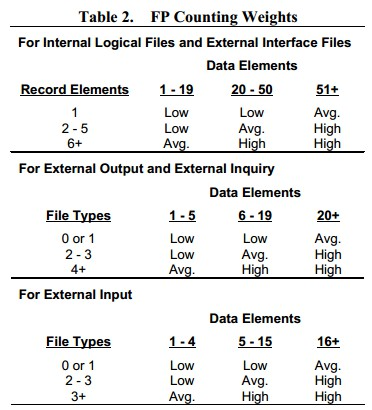
\includegraphics[width=60mm]{img/fpcounting.jpg}}
	\subfigure[UFP Complexity Weights]{\label{fig:fp_total}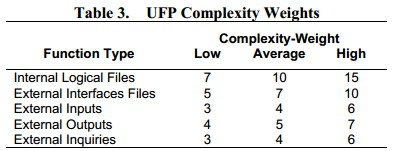
\includegraphics[width=60mm]{img/fptotal.jpg}}
	\caption{FP Analysis}
\end{figure}
\FloatBarrier


\subsection{Internal Logic Files} 

The PowerEnjoy Service needs to store information about:

\begin{itemize}
	\item \textbf{User:} This data consist in a small set of user information, for this reason its complexity has been considered \textbf{Simple}
	\item \textbf{Car:} This data consist in a small set of car information, for this reason its complexity has been considered \textbf{Simple}
	\item \textbf{Safe Area:} This data consist in a small set of safe area information, for this reason its complexity has been considered \textbf{Simple}
	\item \textbf{Trip:} This data consist in a small set of trip information, for this reason its complexity has been considered \textbf{Simple}
\end{itemize}
\fptable{			
	\fprow{User}{0}{7}	
	\fprow{Car}{0}{7}	
	\fprow{Safe Area}{0}{7}
	\fprow{Trip}{0}{7}
}

\subsection{External Interfaces File} 

\begin{itemize}
	\item \textbf{GPS positioning:} This data consist on information received by user or by OnBoard device of the car. \\Because the managing involve some algorithms it's considered \textbf{High}
\end{itemize}

\fptable{			
	\fprow{GPS positioning}{2}{10}	
}

\subsection{External Input} 
\begin{itemize}
	\item \textbf{Sign-Up:} Create a new user entry in the system Database. \\The complexity has been considered \textbf{Simple}
	\item \textbf{Log-In/Log-Out:} Manage the user authentication. Require a module to generate an auth token\\The complexity has been considered \textbf{Medium}
	\item \textbf{Update user information:} Update users information in the system Database. \\The complexity has been considered \textbf{Simple}
	\item \textbf{Request car reservation:} Manage the car reservation in the system. Require many check on the availability.  \\The complexity has been considered \textbf{Medium}
	\item \textbf{Unlock car:} Check if the user is nearby the reserved car and send an unlock request to the car. Require algorithm on user position.  \\The complexity has been considered \textbf{Complex}
\end{itemize}

\fptable{			
\fprow{Sign-Up}{0}{3}	
\fprow{Log-In/Log-Out}{1}{4}	
\fprow{Update user information}{0}{3}	
\fprow{Request car reservation}{1}{4}	
\fprow{Unlock car}{2}{6}
}

\subsection{External Inquiries} 
A PowerEnJoy user can ask the system for the retrieval of some data:
\begin{itemize}
\item \textbf{Car list:} User can request the list of cars available in a certain area or address. Involve Geolocalization algorithms.  \\The complexity has been considered \textbf{Medium}
\item  \textbf{Special Parking Area request:} User can request the list of available special parking areas. Require to query the status of the nearby special parking area.\\The complexity has been considered \textbf{Medium}
\item  \textbf{Parking Area request:} User can request the list of parking areas. Require to query the status of the nearby special parking area. \\The complexity has been considered \textbf{Medium}
\item  \textbf{Personal Data request:} User can request to see its personal data. Data can be obtained with a simple Database Query. \\The complexity has been considered \textbf{Simple}
\item  \textbf{Trip list:} User can request the list of trips done in a certain period.\\
The complexity has been considered \textbf{Complex}
\end{itemize}

\fptable{			
	\fprow{Car list}{1}{4}
	\fprow{Special Parking Area request}{1}{4}
	\fprow{Parking Area request}{1}{4}
	\fprow{Personal Data request}{0}{3}
	\fprow{Trip list}{2}{6}
}

\subsection{External Output} 
Beyond answers to External Inquiries, the system has to send other types of messages to the user:
\begin{itemize}
\item \textbf{Reservation confirmation:} A notification of the confirmation of a reservation. Require email or push notification system. \\The complexity has been considered \textbf{Simple}
\item \textbf{End Trip notification:} A notification of the end of a trip. Require the status of the car through the OnBoard device \\The complexity has been considered \textbf{Medium}
\item \textbf{Payment notification:} A notification of the confirmation of the payment. Require an integration with the payment system \\The complexity has been considered \textbf{Medium}
\end{itemize}

\fptable{			
	\fprow{Reservation confirmation}{0}{4}
	\fprow{End Trip notification}{1}{5}
	\fprow{Payment notification}{1}{5}
}

\subsection{Results} 
According to the element in each section and their weight in complexity the total of  Function Points that provide an indication of the size of the system in functional terms:

\begin{equation}
FP=ILF+EIF+EI+EQ+EO 
\end{equation}

Total Function Points: \textbf{\arabic{total_fp}}


Using 46 as AVC the final value of the estimated line of code is:

\begin{equation}
LOC = 46 * 93 = 4278
\end{equation}

	\pagebreak
	\section{Resources Allocation}
Through a Gantt chart, all activities are represented for blocks over time in order to highlight how resources are allocate to the various tasks. The beginning and the end of the block correspond to the beginning and at the end of the activity. Start of some activities are linked to the end of other.
\\
	\begin{center}
\begin{sideways}

\begin{ganttchart}[
	y unit title=0.5cm,
	y unit chart=0.5cm,
	vgrid={ dotted},
	time slot format=isodate,
	compress calendar,
	today={\the\year-\the\month-\the\day}, 
	title/.append style={shape=rectangle, fill=black!10},
	title height=1,
	bar/.append style={fill=green!90, rounded corners=3pt},
	bar height=.45,
	bar label font=\normalsize\color{black!50},
	group top shift=.6,
	group height=.3,
	group peaks height=.2,
	bar incomplete/.append style={fill=green!40},	
	]{2016-08-01}{2018-05-31}
	\gantttitlecalendar{year} \\
  \gantttitlecalendar{ month} \\



	\ganttset{progress label text={},
		bar incomplete/.append style={fill=green!40},
		group/.append style={draw=black, fill=green},} % this suppresses percentage done labels
	\ganttgroup{Requierements and Design}{2016-10-16}{2017-01-01} \\
	\ganttbar[progress=00, name=rasd]{Requirements Analysis}{2016-10-16}{2016-11-13} \\
	\ganttlinkedbar[progress=00, name=pdd]{Preliminary Design}{2016-11-13}{2016-12-11} \\
	\ganttbar[progress=00, name=itpd]{Integrated Test Plan}{2016-12-11}{2017-01-15} \\
	\ganttbar[progress=00, name=pp]{Project Plan}{2016-12-11}{2017-01-22} \\
	\ganttset{bar incomplete/.append style={fill=red!40},
		group/.append style={draw=black, fill=red}}
	\ganttgroup{Implementation}{2017-2-01}{2017-09-30} \\
	\ganttbar[progress=00, name=impl_database]{Database}{2017-02-01}{2017-03-31} \\
	\ganttbar[progress=00, name=impl_server]{Server Infrastructure}{2017-03-31}{2017-04-30} \\
	\ganttbar[progress=00, name=impl_backend]{Backend Logic}{2017-04-01}{2017-06-31} \\
	\ganttbar[progress=00, name=impl_obsw]{OnBoard Device Software}{2017-05-01}{2017-07-15} \\
	\ganttbar[progress=00, name=impl_app]{Mobile Application}{2017-07-01}{2017-09-30} \\
	\ganttbar[progress=00, name=impl_webd]{Website}{2017-07-01}{2017-09-30} \\
	\ganttset{bar incomplete/.append style={fill=blue!40},
		group/.append style={draw=black, fill=blue},}
	\ganttgroup{Testing}{2017-10-1}{2018-3-31} \\
	\ganttbar[progress=00, name=test_unit]{Unit Test}{2017-10-1}{2017-11-30} \\
	\ganttbar[progress=00, name=test_integration]{Integration Test}{2017-11-30}{2018-1-31} \\
	\ganttlinkedbar[progress=00, name=test_profiling]{Performance Test and Profiling}{2018-02-01}{2018-03-01} \\
	% misc links
	\ganttset{progress label text={}}

	\ganttlink[link mid=0.4]{pdd}{itpd}
	\ganttlink[link mid=0.2]{pdd}{pp}
	\ganttlink[link mid=0.3]{impl_database}{impl_backend}

\end{ganttchart}

\end{sideways}
\end{center}
	\pagebreak
	\section{Risk management}
In this section we mention the risks that could affect our project. We provide a brief description of the risk, its probability to actualize, the impact of such actualization on the project and possible solutions to take into account in order to avoid or limit the damages.
The possible values for the probability are \textit{Low, Medium} or \textbf{High}, while the possible values for the impact are \textit{Marginal, Serious} or \textit{Catastrophic}.
\subsection{Project Risks}
Project Risks are those risks which threaten the project plan and whose actualization can result in a slipping of the schedule \newline
\begin{adjustbox}{max width=\textwidth}
\begin{tabular}{|l|p{5 cm}|l|l|p{5 cm}|}
\hline
Risk & Description & Probability & Impact & Possible Solutions
\\ \hline
Personnel Shortfall & Due to a wrong estimation of the size of the project, there could be not enough people to complete the project deliveries in time & Medium & Serious & Prepare the personnel to the possibility of extra-work due to the lack of people. \newline Plan a possible new recruitment.	 
\\ \hline
Skill Lack & It could be the case that the team hasn't the skill required to face some types of issues, because it was not supposed to deal with them. & Low & Serious & Recruit people with more skills than the strictly required ones. \newline Consider the organization of update courses. 
\\ \hline
Size of the Project & The project size could be underestimated, because of the lack of knowledge about the field of the project  & Medium & Marginal & Prepare more resources than the strictly needed ones. \newline Consider a possible extension of the time of the project
\\ \hline
Competitors & Other companies can begin similar projects & Low & Serious & Plan an additional period in the schedule devoted to the development of new features and the improvement of the quality, in order to discourage the development of other similar projects
\\ \hline
Personnel Illness & People of the staff can be ill in critical phases of the project & High & Marginal & Make some tasks of the staff overlap with each other. In this way there will be always a possible substitute to ill people.
\\ \hline
 Data Loss & Data loss during the development & Low & Critical & Backup strategy and software versioning.
\\ \hline
\end{tabular}
\end{adjustbox}
\subsection{Technical Risks}
Technical Risks are those risks which threaten the quality and the functioning of the product and whose actualization makes the implementation more difficult. \newline
\begin{adjustbox}{max width=\textwidth}
\begin{tabular}{|l|p{5 cm}|l|l|p{5cm}|}
\hline
Risk & Description & Probability & Impact & Possible Solution
\\ \hline
Obsolete Design & Some new technology, that provides so as many better features to force the team to change the design of the system, could born in the course of the project & Low & Serious & Design the system in a way that allows to change components easily.
\\ \hline
Inadequate Infrastructure & The resources, the facilities and the machines provided by the company or owned by the team are discovered to be inadequate for the project & Low & Catastrophic & While defining the budget with the customer, ask him the creation of a fund for possible substitutions of inadequate equipment.
\\ \hline
New Requirements & New requirements are defined after the design phase& Low & Serious &The Waterfall development approach require frozen requirements. Change the to Scrum or Agile approach.

\\ \hline
\end{tabular}
\end{adjustbox}
\subsection{Business Risks}
Business Risks are those risks which threaten the feasibility of a complete product and the chances of selling it. Their actualization can cause bad results on sales and evaluation of consumers. \newline
\begin{adjustbox}{max width=\textwidth}
\begin{tabular}{|l|p{5 cm}|l|l|p{5 cm}|}
\hline
Risk & Description & Probability & Impact & Possible Solution
\\ \hline
Budget Lack & At some point it can be discovered that there has been an underestimation of the costs of project and that the budget is insufficient & Medium & Serious & Prepare a document to deliver to the customer, in which are explained the good results obtained till that moment, the reason for the budget increase, the disadvantages of non-concluding the project and the advantages of improving it with more functionalities.
\\ \hline
Market Risk & The team has developed a good product, but this does not match the real requirements, expectations and needs of consumers, resulting in poor sales & Medium & Catastrophic & Consider interviews to stakeholder and random consumers during all the phases of project in order to have feedbacks on the partial work done till a certain moment.
\\ \hline
\end{tabular}
\end{adjustbox}
	\pagebreak
	\section{Appendix}


	\subsection{Used software}
	\begin{enumerate}
		\item \textbf{TeXstudio:} \url{http://www.texstudio.org/} to redact this document in {\LaTeX} format.
		\item \textbf{Astah:} \url{http://astah.net/} to draw diagrams.		
	\end{enumerate}
	
	
	\subsection{Time effort}
	The estimated time spent by us to redact this document:
	\begin{center}
		\begin{adjustbox}{max width=\textwidth}	
			\begin{tabular}{|l|>{\raggedright}p{15cm}|}
				
				\hline  Andrea Millimaggi & XXh \tabularnewline
				\hline 	Matteo Michele Piazzolla & XXh \tabularnewline
				\hline 		
			\end{tabular}
		\end{adjustbox}
	\end{center}	
	
	
\end{document}



